\chapter{Introduction and Background}

\section{Introduction}

Condensation--the phenomenon whereby a macroscropic number of particles occupy the ground state a system--has been of theoretical and experimental interest for physicists for almost a century. Bose Einstein Condensation (BEC), perhaps the most familiar example, was predicted to occur for a system of non-interacting Bosons at a sufficiently low temperature. This was observed in ultrocold atoms in the 1990s \cite{PhysRevLett.75.3969}, but there are many other examples of condensation, such as Bardeen Cooper Srhrieffer superconductivity \cite{PhysRev.108.1175}. The excitations can even be quasi particles, for example in the case of magnons--electronic spin waves \cite{magnon}.

More recently, another type of quasiparticle, the exciton-polariton, formed from the coupling of electron-hole (exciton) pairs and photons, has been observed to undergo condensation in microcavities \cite{Byrnes2014}. However, to maintain the condensate, the continual pumping of a laser is required, inhibiting the system from attaining equilibrium. Because it cannot, many questions still remain as to the exact nature of the condensate and how the understanding of condensation derived from equilibrium physics must be modified. 

The aim of this project is to address some of these issues by confirming behaviour of the condensate expected from a theoretical analysis. In particular, when describing the condensate as a macroscopic wavefunction $\rho(r,t)e^{i\theta(r,t)}$, it is found that the long range behaviour of the condensate can be described strictly by the evolution of the phase $\theta$ through the Karder-Parisi-Zhang (KPZ) equation \cite{PhysRevX.7.041006,2015PhRvX...5a1017A}. Originally used to describe height growth\cite{PhysRevLett.56.889}, in its current context the compactness of the $\theta$, i.e. that it is limited between $0$ and $2\pi$, allows for the existence of topoligal defects which are crucial in explaining the physics.

By employing techniques from the renormalistion group, it is found that depending on the parameters of the equation there are effectively two regimes \cite{PhysRevX.7.041006,2015PhRvX...5a1017A}. The first is described by Berezinskii-Kosterlitz-Thouless (BKT) physics, which is that of the $XY$ model. The second, the KPZ phase. 
During the porject, the evolution of the condensate phase was simulated through the KPZ equation, to confirm that in the different regime the behaviour was as expected. 


\section{Exciton-Polariton Condensates}

Exciton-polaritons are formed in a laser illuminated microcavity--an example of a so-called drive dissipative system: the laser contiually \emph{drives} the microcavity and photons inside the cavity escape or 
\emph{dissipate} continually out of the microcavity. As such, the system is distinctly non equilibrium due to the external influence. 

To create these quasiparticles, a thin superconducting surface is sandwitched between two reflective Bragg mirrors on either side. The material is then illuminated with a laser, exciting an electron, which, because of the Coulombic interaction, forms a hydrogen-like bound state with the remaining hole: an exciton. The excitons are also confined to very narrow widths in the material due to the alternating doping that varies the band gap, making the system two dimensional. This is illustrated in \fig{\ref{fig:exciton-polariton}}. Perpendicular to the surface \cite{doi:10.1080/00107514.2010.550120}, the photon wavevector is restricted due to the finite length $L$ of the $z$ plane, the possible values given by $2\pi N/L$ where $N$ is an integer. The possible frequencies are therefore 
\[
\omega = \frac{c}{n}\sqrt{k^2 + (2\pi N/L)^2} 
\]
where $n$ is the material refractive index and $k$ is the magnitude of the `in-plane' wavevector. If this is small, we may expand this dispersion to obtain
\[
\hbar \omega = \hbar \omega_0 + \hbar^2k^2/2m 
\]
where $m = \hbar(n/c)(2 \pi N /L)$ is the effective mass of the photon and is set by the cavity length. The energy  $\omega_0 = (c/n)(2 \pi N / L)$ at the bottom of the dispersion should be near to that of the energy rquired to create an exciton. This fixes the photon mass to be $m \sim 10^{-4}m_e$ while the exciton mass is typically $\sim m_e$, meaning we can neglect the exciton dispersion compared to that of the polariton. 

\begin{figure}[htbp!]
	\centering
	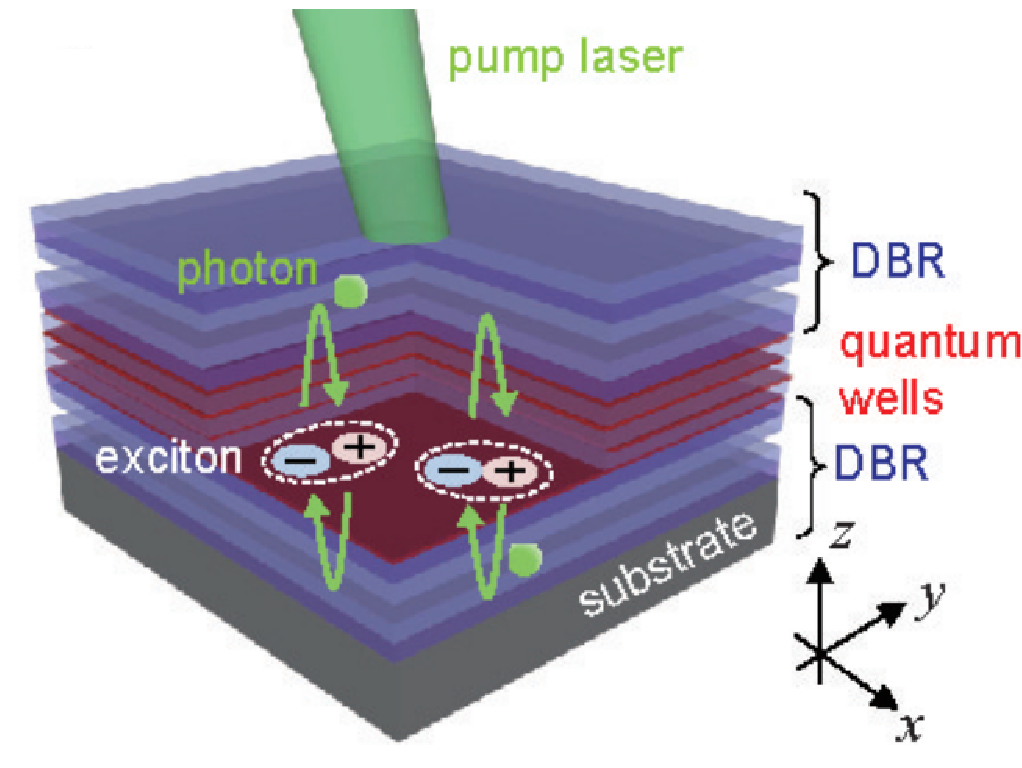
\includegraphics[scale=0.4]{./Figures/polaritonsystem.pdf}
	\caption{The exciton-polariton microcavity.
	Superconducting material of with an alternating band gap is sandwiched between Bragg mirrors. 
	A laser illuminates the semiconducting material which creates excitons that are confined in a 2D plane due to the doping. 
	With sufficient photon lifetime, the photons can couple with the exciton, effectively becoming a quasi particle known as a exciton-polariton \cite{Byrnes2014}.}
	\label{fig:exciton-polariton}
\end{figure}

Although the mirrors are not perfectly reflective,
with the lifetime of the polaritons being limited to $\sim 200 ps$ in current experiments \cite{2014arXiv1408.1680S}, if the rate of recombination and electron excitation exceeds that of photon dissipation,
the excitons are able to couple with the photons. To describe this \cite{RevModPhys.85.299}, the Hamiltonian of the photons is given by 
\[
\mathcal{H}_{\text{cav}} = \int \frac{\dd[2]{\myvec{k}}}{(2\pi)^2} \sum_\sigma 
\hbar\omega_{\text{cav}}(\myvec{k})\hat{a}^\dagger_{C,\sigma}(\myvec{k})\hat{a}_{C,\sigma}(\myvec{k})
\]
where $\hat{a}^\dagger_{C,\sigma}(\myvec{k})$ is the Bosonic creation operator for a photon with in-plane wavevector $\myvec{k}$ and polarisation $\sigma.$ The exciton Hamilotian is given by 
\[
\mathcal{H}_{\text{exc}} = \int \frac{\dd[2]{\myvec{k}}}{(2\pi)^2} \sum_\sigma 
\hbar\omega_{\text{exc}}(\myvec{k})\hat{a}^\dagger_{X,\sigma}(\myvec{k})\hat{a}_{X,\sigma}(\myvec{k})
\]
with analogous definitions. The interaction Hamiltonian is then 
\[
\mathcal{H}_{\text{int}} = \int \frac{\dd[2]{\myvec{k}}}{(2\pi)^2} \sum_\sigma \hbar \Omega_R [ \hat{a}^\dagger_{X,\sigma}(\myvec{k})\hat{a}_{C,\sigma}(\myvec{k}) + \hat{a}^\dagger_{C,\sigma}(\myvec{k})\hat{a}_{X,\sigma}(\myvec{k})]
\]
describing the interconversion of photons and excitons, with the strength given by the Rabi frequency $\Omega_R$. Defining 
\[
\hat{\myvec{a}}_\sigma(\myvec{k}) = 
\begin{pmatrix}
\hat{a}_{C, \sigma}(\myvec{k}) \\
\hat{a}_{X,\sigma}(\myvec{k})
\end{pmatrix}
\]
we can write the total Hamiltonian by 
\[
\mathcal{H} = \int \frac{\dd[2]{\myvec{k}}}{(2\pi)^2} \sum_\sigma \hat{\myvec{a}}_\sigma (\myvec{k})^TM(\myvec{k}) \hat{\myvec{a}}_\sigma(\myvec{k})
\]
where $M(\myvec{k})$ is given by 
\[
\begin{pmatrix}
\hbar\omega_{\text{cav}}(\myvec{k}) & \hbar \Omega_R \\
\hbar \Omega_R & \hbar\omega_{\text{exc}}(\myvec{k})
\end{pmatrix}.
\]
Diagonalising, we see that the frequencies of the eigenfunctions, which are linear combination of the exciton and photon creation operators (exicton-polaritons), is given by
\[
\omega_{\text{(UP,LP)},\sigma}(\myvec{k}) = \frac{\omega_{\text{cav},\sigma}(\myvec{k}) + \omega_{\text{exc},\sigma}(\myvec{k})}{2} \pm \left[ \Omega_R^2 + \left(\frac{\omega_{\text{cav},\sigma}(\myvec{k}) - \omega_{\text{exc},\sigma}(\myvec{k})}{2}\right)^2\right]^{1/2}
\]
where `UP' and `LP' stand for upper and lower polariton, respectively. As mentioned, the exciton dispersion is very flat compared to the photon. Thus, the polariton dispersion is almost totally dependent on the photon. At low frequencies the LP dispersion is approximately quadratic but has a point of inflection as the momentum is increased and approaches the exciton dispersion. During laser puming it is the LP modes that are occupied. 

\begin{figure}[htbp!]
	\centering
	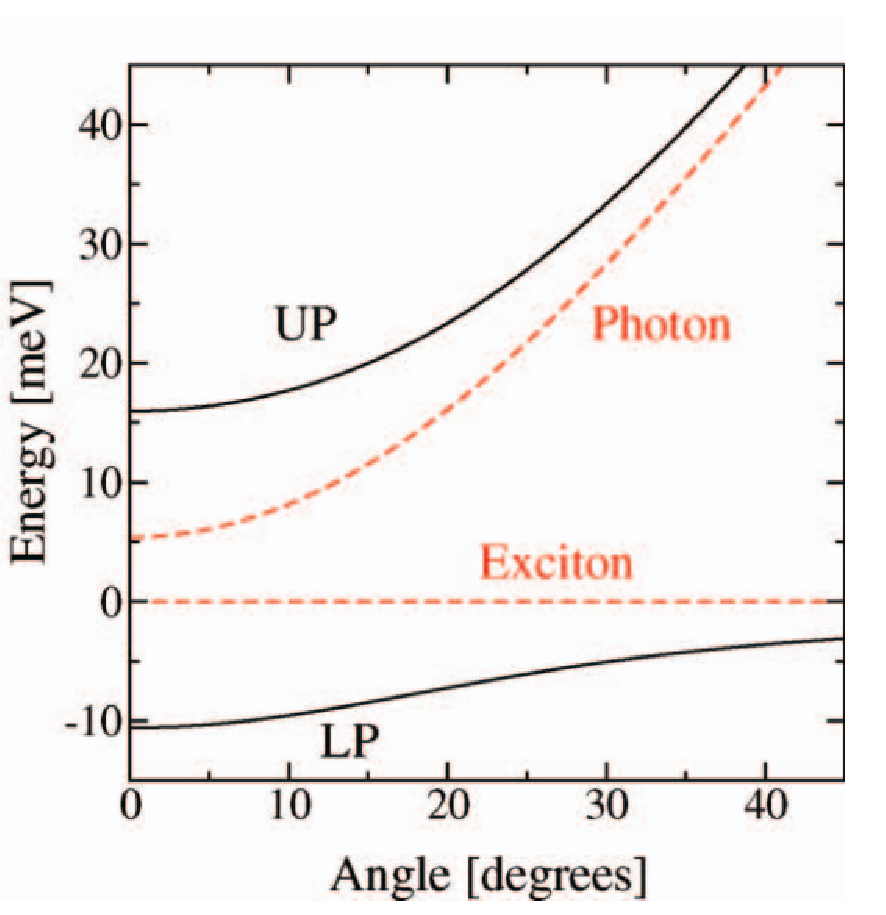
\includegraphics[scale=0.4]{./Figures/polaritondispersion.pdf}
	\caption{A dispersion graph for the exciton-polariton system. The angle corresponds to the momentum of the polariton. LP and UP are upper and lower polariton, respectively, and are the two eigenvalues for the Hamiltonian. Due to the photon's low effective mass compared to the exciton, the dispersion for the polariton is almost totally dependent on the photon dispersion. In experiments it is the LP modes that are become occupied. Its dispersion relation looks quadratic at low momentum but has a point inflection, tending to the exciton dispersion, at high momentum. \cite{doi:10.1080/00107514.2010.550120}}
	\label{fig:polaritondispersion}
\end{figure}

One can obtain a wide range of behaviour in the microcavity by varying the method of illumination. 
The momenta of the created polaritons in the microcavity plane depends on the $\sin \theta$ where $\theta$ is the angle of the laser with respect to the plane \cite{doi:10.1080/00107514.2010.550120}. 
To obtain a condensate where a low momentum mode is macroscopically occupied, there a few standard methods, two of which we will describe, however in general they depend on the pump strength, and, after a level has been passed, accumulation of the low momentum states increases dramatically.

The first of these is the incoherent pump. Here the laser excites high momentum polaritons. These can decay through phonon scattering at first, but as the dispersion steepens this process becomes more and more inefficient and this creates a bottle-neck effect near the inflection. However, if the density of the polaritons is high enough then polariton-polariton scattering can take over, scattering the polaritons to high and low momentum states, the high momentum states then repeating this process. By ensuring the polariton is more exciton-like, so that their interactions are strengthened, and that the density is high enough, this process leads to the formation of the condensate \cite{doi:10.1080/00107514.2010.550120}.

The second method is the coherent pumping scheme which leads to opitical parametric oscillation. This is a `cleaner' method. Here the pump is tuned at the inflection point and so any subsequent polariton interaction can cause scattering of two low and high momentum states which conserve both momentum and energy, known as the signal and idler modes, respectively. The idler can then decay to the lower momentum state via phonon emission. Beyond a threshold pump power the density of the low and high momentum states increases \cite{doi:10.1080/00107514.2010.550120}.

These techniques allow experimenters to observe a BEC, for example in \cite{PhysRevLett.118.016602}, and illustrated in \fig{\ref{fig:polariton-condesation}}. 

\begin{figure}[htbp!]
	\centering
	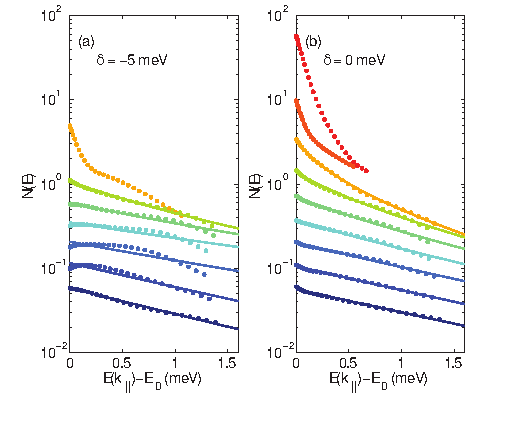
\includegraphics[scale=1]{./polaritoncondensation.pdf}
	\caption{From \cite{PhysRevLett.118.016602}, the energy distribution of polaritons at two detunings $\delta$ (which is the energy difference between the cavity resonance and exciton energy at $k=0$) and various pump powers, shown here as increasing when going from blue to red. For zero detuning at a sufficient pump power, the distribution unambiguously points to Bose-Einstein statistics.}
	\label{fig:polariton-condesation}
\end{figure}


In general, however, condensation is not necessarily indicative of the system being a BEC. 
Various regimes are possible where the system behaves more like a laser, a distinctly non-equilibrium system, or like a BEC as above.
It is thus most fruitful to consider the system as lying somewhere on a spectrum from the laser of BEC system \cite{Byrnes2014}. When condensation occurs, it is possible consider a macroscopic wavefunction $\psi(\myvec{r},t)$ of the system, which can also be written as $\sqrt{\rho(\myvec{r},t)}e^{i\theta(\myvec{r},t)}$ where $\rho(\myvec{r},t)$ is the (real) amplitude and $\theta(\myvec{r},t)$ is the phase.

We will look more in detail about the dynamics and phases of this condensate, but first we must discuss a related model.


\section{$XY$ model and the BKT transition}

The two dimensional $XY$ model consists of a finite lattice of unit length spins that can rotate freely rotate the plane of the lattice \cite{altland2010condensed}. The Hamiltonian describing the system is given by 
\[ 
\mathcal{H} = -J\sum_{\left <i,j \right>} \sum_{\{x,y\}} \myvec{s}_{i,j} \cdot \myvec{s}_{i+x,j+y} =
    -J\sum_{(i,j)} \sum_{\{x,y\}}  \cos( \theta_{i,j} - \theta_{i+x,j+y}) 
\]
 where $i, j$ signifies point $(i,j)$ and $\{x,y\}$ are the pairs $\{0,1\} \{0,1\}$, i.e. nearest neighbours, and $J$ is a constant. Periodic boundary conditions have been employed. We can form the continuum long wavelength (slowly varying) version of this equation by expanding in a Taylor series and keeping only terms to second order (as higher order terms will have Fourier transformed components greater than $k^2$ and we are ignoring those)
 \[
 -J\sum_{(i,j)} \sum_{\{x,y\}} \left ( 1 - \frac{a^2}{2} \frac{( \theta_{i,j} - \theta_{i+x,j+y})^2}{a^2} \right).
 \]
The first term is a constant that can be ignored in what follows. Taking $a \to 0$, we have that $\sum_{(i,j)} a^2 \to \int \dd{x}\dd{y}$ and the terms in brackets become partial derivative, i.e. we obtain
 \[
 \frac{J}{2} \int \dd{x} \dd{y} (\nabla \theta)^2
 \]
 where now $\theta$ is a continuous variable. The Hamiltonian under consideration is invariant under global SO(2) transformation, i.e. in the replacement of $\theta \to \theta + \delta \theta$ as the change in cancelled in the $\cos$ terms. Because the system is two dimensional and interacting, it is impossible for the symmetry to be spontaneously broken, that is, the system cannot occupy a state in which all the spins point in the same direction \cite{Coleman1973}. To demonstrate this, we will show that $\mean{(\theta(\myvec{r})\theta(\myvec{0}))^2}$ diverges as $r \to \infty$, which means the fluctuations between the origin and $\myvec{r}$ diverges as $r \to \infty$, so there can be no long range order \cite{8.334 lecture notes}. We note that the probability of a configuration is given by 
 \[
  \mathcal{P}[\theta(\myvec{r})] =   \exp \left [   -\beta J/2 \int \dd[2]{\myvec{r}} (\nabla \theta)^2 \right ]
 \] 
 If instead we decompose  $\theta$ into its Fourier decomposition $\theta(\myvec{r}) = \sum_{\myvec{k}} \theta_{\myvec{k}} e^{i \myvec{k}\cdot \myvec{r}}$ where the sum is over the Brillouin zone, we then obtain for the probability of $\theta_{\myvec{k}}$
 \[
 \mathcal{P}[\theta_{\myvec{k}}] = \exp \left[-\beta J L^2/2 k^2 |\theta_{\myvec{k}}|^2 \right]
 \]
 where $L^2$ denotes the system size and we use $\theta_{\myvec{k}} = \theta_{\myvec{-k}}^*$. Now $|\theta_{\myvec{k}}|^2 = (\Re \theta_{\myvec{k}})^2 + (\Im \theta_{\myvec{k}})^2$ and we can write the probability of a configuration as 
 \[
 \begin{split}
 \mathcal{P}[\{\theta_{\myvec{k}}\}] &= \prod_{\myvec{k}} \exp \left[-\beta J L^2/2 k^2 |\theta_{\myvec{k}}|^2 \right] \\ &=\prod_{\myvec{k}, k_x > 0} \exp \left[-2\beta J L^2/2 k^2((\Re \theta_{\myvec{k}})^2 + (\Im \theta_{\myvec{k}})^2) \right]
 \end{split}
 \]
 where in the second we restrict ourselves to the positive $x$ and thus obtain completely decoupled Gaussian variables with variance $1/\beta J L^2$. Then the variances of $\theta_{\myvec{k}}$ are given by 
 \[
 \mean{\theta_{\myvec{k}} \theta_{\myvec{k}'}} = \mean{\Re \theta_{\myvec{k}} \Re \theta_{\myvec{k}'}} + \mean{\Im \theta_{\myvec{k}} \Im \theta_{\myvec{k}'}} = \delta_{\myvec{k}, \myvec{-k'}}/\beta J L^2 
 \]
 We wish to calculate 
 \[
 \mean{\theta(\myvec{r})\theta(\myvec{r}')} = \sum_{\myvec{k}, \myvec{k'}} e^{i \myvec{k} \cdot \myvec{r} + i \myvec{k}' \cdot \myvec{r}'} \mean{\theta_{\myvec{k}} \theta_{\myvec{k}'}} = \frac{1}{\beta JL^2}\sum_{\myvec{k}} \frac{e^{i \myvec{k} \cdot( \myvec{r} - \myvec{r}')}}{k^2}
 \]
 which can be replaced by an integral by $1/L^2 \sum_{\myvec{k}} \to \int \dd[2]{\myvec{k}}/(2\pi)^2 $ so that we obtain
 \[
 \frac{1}{\beta J} \int \frac{\dd[2]{\myvec{k}}}{(2 \pi)^2} \frac{e^{i \myvec{k} \cdot( \myvec{r} - \myvec{r}')}}{k^2}.
 \]
 The negative of the integral is the Green's function of $\nabla^2$:
 \[
 -\int  \frac{\dd[2]{\myvec{k}}}{(2 \pi)^2} \nabla^2 \frac{e^{i \myvec{k}.(\myvec{r} - \myvec{r}')}}{k^2} = \int  \frac{\dd[2]{\myvec{k}}}{(2 \pi)^2} k^2 \frac{e^{i \myvec{k}.(\myvec{r} - \myvec{r}')}}{k^2} = \delta^2(\myvec{r}-\myvec{r}')
 \]
 A solution $V$ depends only on $|\myvec{r}-\myvec{r}'|$ as the integrand has an inner product with $\myvec{k}$ which takes on all values, so we can find $V$ with the divergence thoerem:
 \[
 \int \nabla \cdot \nabla V\dd[2]{\myvec{r}} \int r \nabla V \dd{\Omega} = 2 \pi r \nabla V  = 1. 
 \]
 With $\nabla V = \pdv*{V}{r}$  this is $V(r) = \ln(r)/2\pi +C$. Now $\mean{(\theta(\myvec{r}) - \theta(\myvec{r}'))^2}$ = 
 \[
 2\mean{\theta(\myvec{r})^2} - 2\mean{\theta(\myvec{r})\theta(\myvec{r}')}.
 \]
We also have $\mean{\theta(\myvec{r})}=0$ as it is the sum of the Gaussian distributed variables. Since the range of $\theta$ is no longer $[0,2\pi]$ in this analysis, we interpret the mean of $\theta$ being 0 and the variance infinite in that it can occupy any value with equal probability, as there is no preference for a direction. Clearly due to our simplification there will be undefined behaviour, so we set 
\[
 2\mean{\theta(\myvec{r})^2} - 2\mean{\theta(\myvec{r})\theta(\myvec{r}')} =  \frac{\log(|\myvec{r} - \myvec{r}'|/a)}{\beta J  \pi}
\]
where $a$ is of the order of the lattice spacing ensuring the $\log$ is unitless. We have ignored the infinite constant. From this result we see that the correlations diverge as $|\myvec{r} - \myvec{r}'| \to \infty$.  For free, we can calculate the spin correlations in space $\mean{\cos \theta(\myvec{r} - \myvec{r}')}.$ We use 
 \[
 \mean{e^{A}} = e^{\left(\mean{A} + \tfrac12 \mean{A^2}\right)}.
 \]
Thus, the correlations in space are of the form
\[
\mean{\cos \theta (\myvec{r} - \myvec{r}')} = \Re \mean{e^{i\theta (\myvec{r} - \myvec{r}')}} \propto \frac{1}{|\myvec{r}- \myvec{r}'|^{\eta}}
\]
for an exponent $\eta$. We then see that while there is no spontaneous symmetry breaking, there still exists a phase with `algebraic' decay of correlations. Since in making the continuum assumption we only retained the leading order term in the Taylor expansion, we are implicitly assuming assuming large $
\beta J$ that penalises large fluctuations of the spins \cite{altland2010condensed}. This is the low temperature phase. Assuming $\beta J$ small, we may expand the exponential of the original Hamiltonian in powers of $\beta J$ so that the partition function approximately: 
\[
\mathcal{Z} = \int  \prod_{\myvec{r}} \dd{\theta(\myvec{r})} \prod_{\myvec{r}'} [1 + \beta J \cos(\theta(\myvec{r}) - \theta_(\myvec{r}')) + \mathcal{O}(J^2
)]\]
In determining the correlations in this regime, we note that any integral of the form 
\[
\int_{0}^{2\pi} \dd{\theta_k} \cos(\theta_i -\theta_j) 
\]
is zero whereas
\[
\int_{0}^{2\pi} \dd{\theta_k} \cos(\theta_i -\theta_j)\cos(\theta_j - \theta_k)= \pi \cos(\theta_i - \theta_k)
\]
Thus for the correlation we have 
\[
\mean{\cos(\theta(\myvec{r})- \theta(\myvec{0}))} \propto (\pi J)^{|\myvec{r}|}
\]
as there is an order $|\myvec{r}|$ of cosine terms in the product that are required to `connect' $\myvec{0}$ to $\myvec{r}$. 
We may rewrite this expression as $\exp[-|\myvec{r}|/\xi]$ where $\xi^{-1} = 1/\pi \beta J$ and is the `correlation length' of the system. It quantifies the distance that the spins are correlated. This intuitive approach has revealed that, in high temperature phase, the correlations decay exponentially. The two types of decay -- algebraic and exponential -- are hallmarks of two phases in certain 2D systems, and the transition between the two is known as the BKT transition. More rigorous analysis reveals that the correlation length diverges at the critical point of the transition, and tends to zero as one moves away in either direction. 

What differentiates the two phases? The main insight is that the system enables the existence of topoligcal defects known as `vortices'. This means that we cannot continuously deform a state with vortices into one without them, and thus it cannot be obtained through perturbation theory. To see their origin, note that the phase at each point is restricted to $[0, 2\pi]$,  i.e. it is compact, and so the circulation, defined by 
\[
\int \nabla \theta \cdot \dd{\myvec{l}} = 2\pi n
\]
must be restricted to $2 \pi n$ where $n$ is an integer so that the phase angle is not multiple valued. Now by the gradient theorem we know that if the gradient is everywhere defined inside the loop then this loop integral should be zero, already signaling that there must be a singularity for vortices to exist. Phase transitions are manifested by singularities in various quantities, and it is indeed it is in the absence or presence of vortices that is indicative of the phase the system occupies. 

To obtain a better intuition for the subject, let us consider an isotropic solution $\nabla \theta = \frac{n}{r} \myvec{\hat{r}}$. The integer $n$ is known as the charge of the vortex, as then the solution is $\theta(\myvec{r}) = \log(r)$ which describes a Coulombic charge in two dimensions. This provides a revealing picture for the system: in the low temperature phase the `charges' are bound, but increasing the temperature beyond the transition is marked by an unbinding and proliferation of these vortices. Since the free energy $F = U - TS$ is minimised at a given temperature and volume, the proliferation at the critical point must mean the entropy increase is more favourable than the energy increase. 

To estimate both, imagine that we have one vortex in the system. We use our expression for the energy
\[
\int \dd[2]{\myvec{r}} | \nabla \theta |^2 \propto \log(L)
\]
where $L$ is the system size. The number of places to put the vortex is proportional to $L^2$, so the entropy $k \log \Omega$ must also be proportional to $\log L$. As both have this proportionality, it is then clear that, at the critical point, $U - T_cS$ makes vortex proliferation favourable. All these points will come into play in a modified form in the study of polariton condensates.

After considering equilibrium issues, what of dynamics? We describe \cite{2016PhRvB..94j4521S} the evolution of $\theta_{i,j}$ according the Langevin equation 
\[
\partial_t \theta_{i,j} = -\Gamma \frac{\delta \mathcal{H}}{\delta \theta_{i,j}} + \eta=-\Gamma \pdv{\mathcal{H}}{\theta_{i,j}} + \eta
\]
where $\eta$ is a Guassian white noise term $\mean{\eta(\myvec{r},t), \eta(\myvec{r}',t')} = 2 \Delta \delta(t-t')\delta(\myvec{r}-\myvec{r}')$. In the discrete version this is
\[
\partial_t \theta_{i,j} = +\Gamma J \sum_{\{x,y\}} \sin(\theta_{i,j} -\theta_{i+x,j+y})
\]
where $\{x,y\}$ are as before. The continuum version of this equation requires $\delta \mathcal{H} / \delta \theta$ which is 
\[
\frac{\delta \mathcal{H}}{\delta \theta} = \frac{J}{2} \int \dd[2]{\myvec{r}}  2 (\nabla \theta)(\nabla \delta \theta).
\]
Intgerating by parts we find that the integrand is zero for $J\nabla^2 \theta$ so the equation is 
\[
\partial_t \theta = -\Gamma J \nabla^2 \theta + \eta.
\]

We will see that this is the equation of our system describing the long wavelength behaviour of the condensate phase when we are in a certain regime.

\section{$XY$ model scaling violations}

To understand the approach taken in the project, we describe the approach taken in \cite{PhysRevLett.84.1503} to determine dynamical evolution of the correlation length $\xi$ as the system $XY$ system is quenched from the disordered (high temperature) phase to the ordered (low temperature) phase. Using renormalisation group methods \cite{Janssen1989}, the dynamical exponent $z$ is predicted to be 2 so that the correlation length grows as $\xi(t) = t^{1/2}$ and $t$ is a substitute of the relaxation time of the system to the evolution of the system. The relaxation time also diverges at criticality, known as `critical slowing down' \cite{nishimori2011elements}. 
To test this prediction, for various system sizes a plot of the time dependent Binder cumulant defined by 
\[
g_L(t) = 2 - \frac{\mean{\myvec{M}^2}^2}{\mean{\myvec{M}^4}}
\]
was plotted where $\myvec{M}(t)$ is the magnetisation (the average of $(\cos \theta_{i,j},\sin\theta_{i,j})$ on the lattice. The mean of $\myvec{M}$ is over independent Monte Carlo realisations. In a disordered condition where each spin is random, each component magnetisation is the sum of independent uniformly distributed numbers, and so by the central limit theorem are approximately Gaussian distributed. Then $\mean{\myvec{M}^2}^2/\mean{\myvec{M}^4}$ is 2, so $g_L$ is 0. In an ordered state where all spins are aligned, the ratio is one, and $g_L$ is 1. The Binder cumulant is thus a convenient quantity to act as an ordered parameter.

Crucially, it is dimensionless. Therefore, for different system sizes, plotting the Binder cumulant as a function of another dimensionless quantity should result in all the curves `collapsing' into one. Since we are varying the system size $L$, the ratio $\xi^2/L^2 = t/L^2$ is appropriate. 

This was done in two cases: first in the quench from a completely ordered phase to one below the critical temperature, where $z=2$ provided a good collapse. In the quench from the random initial condition to the ordered phase, however, a much higher exponent $z=2.35$ was required to achieve the same quality in collapse. The disparity was explained by the requirement of vortex-antivortex binding necessary when queching from the disordered initial condition, which slows the approach to equilibrium. Indeed, a modification of the functional form of $\xi$ was found to be necessary, and was $\xi(t) = (t/\log(t/t_0))^{1/2}$. The collapse is shown in \fig{\ref{fig:xyscaling}}.

\begin{figure}[htbp!]
	\centering
	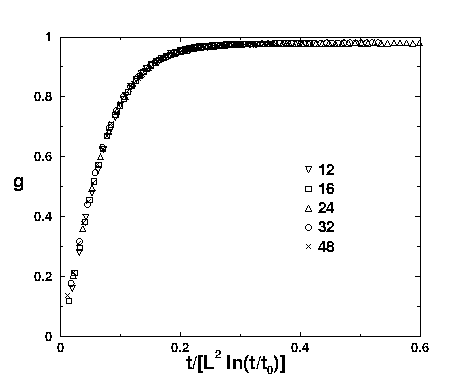
\includegraphics[scale=0.9]{./xyscaling.pdf}
	\caption{Scaling violation of the Binder cumulant $g$ when quenching from the disordered phase to the critical temperature. 
	Rather than standard scaling form $\xi \propto t^{1/z}$ ($z$ being 2 when quenching from the ordered phase), it is modified by $\xi \propto (t/\ln(t))^{1/2}$ due to vortex interactions \cite{PhysRevLett.84.1503}.}
	\label{fig:xyscaling}
\end{figure}

The physical origin of this was in the friction and attraction experienced by the vortices. For the attraction, we found earlier that the vortices behave as 2D Coulombic charges, and thus the force between them is proportional to $1/R$ where $R$ is the vortex distance. The friction was determined from the evolution equation (without noise, or $T=0$), i.e. $\partial_ \theta = -\delta H/ \delta 
\theta$ (the prefactors being set to 1). If $\theta(x,y,t)= \theta_v(x-vt,y)$ is the vortex motion is now
\[
\dv{E}{t} = \int \dd[2]{\myvec{r}} \frac{\delta E}{\delta \theta}\pdv{\theta}{t} = - \int \dd[2]{\myvec{r}} \left(\pdv{\theta}{t}  \right)^2 = -v^2 \int \dd[2]{\myvec{r}} \left( \pdv{\theta_v}{x}\right)^2
\]
Now for a frictional force $-\gamma \dot{x}$ we see that the last integral must be the friction constant. Using the equilibrium vortex configuration we found earlier, which is isotropic, and hence we replace the derivative by $x$ with the gradient, we see that the zero velocity vortex friction is the equilibrium energy, and thus scales like $\log R$, the vortex distance. 

Taking the correlation length as the vortex distance, the velocity of the vortices is $\dv*{\xi}{t} \sim F/\gamma \sim 1/(\xi \log \xi)$ so that $\xi \sim (t/\log t)^{1/2}$. 

\section{Mapping to the KPZ Equation}

We now in see what way our polariton condensate relates to the $XY$ model. Previously we discussed two pumping regimes for the microcavity: incoherent and the OPO regimes. The long wavelength dynamics of the phase in both cases is governed by the compact anisotropic KPZ equation \cite{PhysRevX.7.041006}
\[
\partial_t \theta = D_x \pdv[2]{\theta}{x} + D_y \pdv[2]{\theta}{y} + \lambda_x \left(\pdv{\theta}{x}\right)^2  + \lambda_y\left( \pdv{\theta}{y}\right)^2 + \eta
\]
where $\eta$ is the Gaussian white noise term as before. We see that if the $\lambda$s are set to zero (the $D$s can always be set to one by rescaling the coordinates) we reobtain the equation for the $XY$ model evolution.

However, the physical origin and the interpretation of $\theta$ is different in both cases, which will be discussed. First, as we described earlier the polariton system can form a condensate by adjusting the drive parameters appropriately, and hence we can describe the condensate by a macroscopic wave function $\rho(\myvec{r})e^{i \theta(\myvec{r})}$. Since the phase angle is compact, by the same arguments as before, vortices are allowed to exist. 

In the incoherent pump regime the dynamics of the condensate can be phenomenologically described by the dissipative Gross-Pitaevskii equation \cite{2015PhRvX...5a1017A}
\[
\partial_t \psi(\myvec{r}, t) = - \frac{\delta H_d}{\delta \psi^*} + i\frac{\delta H_c}{\delta \psi^*} + \eta
\]
where $H_d$ and $H_c$ are responsible for the coherent and dissipative dynamics and are given by 
\[
H_l = \int r_l |\psi|^2 + K_l^x|\partial_x \psi|^2 + K_l^y|\partial_y \psi|^2 + \tfrac12 u_l |\psi|^4
\]
where $l=\{c, d\}$. The last term is a complex Gaussian white noise. The equation then reads
\[
\partial_t \psi = -r_\text{eff}\psi +K^x_{\text{eff}}\partial_x^2\psi +K^y_{\text{eff}}\partial_y^2\psi -u_{\text{eff}}|\psi|^2\psi + \eta
\]
where $A_{\text{eff}} = A_d -iA_c.$ To simplify this equation, and in particular to determine an equation only dependent on $\theta$, the condensate is expanded about a mean $(M_0 + \chi)e^{i\theta}$ where $M_0$ is set to be a static and uniform solution when $\eta = 0$ and $\theta=0$. This gives $r_{\text{eff}}M_0 = -u_{\text{eff}}M_0^3$. The coeffient $r_c$ is arbitrary and can be set by a local and time dependent transformation $\psi' = \psi e^{i \omega t}$, and this freedom is used to set $r_c = -u_cM_0^2$ and $r_d = -u_dM_0^2$. The physical origin of the other terms is as follows: $r_d$ is the particle loss rate less the pump rate. Clearly the loss rate depends on the density of polaritons, and in the incoherent regime a sufficient density is required for polariton creation. The $K_c$ terms are the momentum coefficents in the $x$ and $y$ directions, inversely proportional to $m_x$ and $m_y$, while $K_d$ are diffusion-like terms. Finally, the $u_c$ term describes a two polariton interaction, and $u_d$ is also a loss term but is non linear. The latter ensures that the polariton density does not grow without bound. 

Substituting the mean expansion and linearising the $\chi$ fluctuation (also ignoring terms like $\partial_x \chi \partial_x \theta$), gives
\[
\partial_t \chi = -2u_d M_0^2 \chi - K_c^x M_0 \partial_x^2 \theta -K_c^y M_0 \partial_y^2 \theta - K_d^x M_0(\partial_x \theta)^2 -K_d^y M_0(\partial_y \theta)^2 + \Re \eta
\]
\[
M_0\partial_t \theta = -2u_c M_0^2 \chi + K_d^x M_0 \partial_x^2 \theta +K_d^y M_0 \partial_y^2 \theta - K_c^x M_0(\partial_x \theta)^2 -K_c^y M_0(\partial_y \theta)^2 + \Im \eta
\]
where the real and imaginary parts were equated. In the low frequency limit, the left hand side is negligible compared to the first term on the right as as it has a time derivative, therefore can be ignored in when $\omega \to 0$. The first equation can then be solved for $\chi$ and substituted into the second, from which the KPZ equation is obtained. That the long wavelength limit results in only $\theta$ dependence is as expected as the U(1) symmetry (clear from the Hamiltonian) means that the excitation about small $k$ is `gapless' in that the energy of the excitation tends to zero (since a slowly varying rotation in space can be made to require arbitrarily small energy). In contrast, excitations of the other variables are `gapped' and the dispersion does not tend to zero at low $k$ but some finite value as there is no corresponding symmetry. Thus we need only retain $\theta$ dependence.

For the coherent pump regime, purportedly the same dynamics is followed. However, here an \emph{ab initio} rather than phenomlogical model is possible, and the meaning of $\theta$ is different: $\theta = \theta_s - \theta_i$ where $s$ and $i$ stand for the signal and idler modes. There again exists a U(1) symmetry as now polariton scattering is described by terms such as $\psi_s\psi_i{\psi_p^*}^2 + \text{h.c.}$ which are invariant under a transformation $\psi_s \to \psi_se^{i\alpha}$, $\psi_i \to \psi_ie^{-i\alpha}$, and $\psi_p$ kept the same. This symmetry
results in a gapless excitation and the KPZ equation is obtained with the modified $\theta$.

To obtain the discretised version of this equation \cite{PhysRevB.94.10452}, the linear terms are transformed as before in the $XY$ model, i.e. by 
\[
\partial_x^2 \theta_{i,j}  = -\sum_{x=\{-1,1\}} \sin(\theta_{i,j} - \theta_{i+x,j})
\]
and analogously for the $y$ direction. The nonlinear terms are the second order coefficients in the expansion of $\cos$, so the prescription for these is
\[
(\partial_x \theta_{i,j})^2  = -\sum_{x=\{-1,1\}} (\cos(\theta_{i,j} - \theta_{i+x,j})- 1)
\]
and analogously for the $y$ direction. There is no factor of 2 as we are summing two such $\cos$ terms in each case. 

\section{Polariton Condensate Regimes}

Using the KPZ equation parameters, the regimes of the condensate are parametrised \cite{PhysRevX.7.041006} by the scaled nonlinearity \[
g \equiv \lambda_x^2/D_x^2\sqrt{D_xD_y}
\]
and the scaled anisotropy
\[
\Gamma = \lambda_y D_x/\lambda_x D_y.
\]
For the KPZ equation to be stable, the $D$s must be positive. The sign of the anisotropy therefore depends on the signs of the $\lambda$s, and only their relative sign matters. The cases $\Gamma > 0$ and $\Gamma <0$ are called the weak and strong anisotropic phases, respectively. 

To determine the long range behaviour in the absense of vortices, rernormalisation group (RG) analysis has been peformed. The essential idea is as follows: over small length scale the system is course grained so is in a sense averaged. A microscropic length scale of the system (such as lattice spacing) is then obtained by shrinking the course grained length scale down to the lattice spacing. This process results in a new description of the system with the parameters adjusted. After repeated application of this procedure, a `flow' of the parameter values is obtained (essentially a phase portrait) and the terms that are non zero at the fixed points, which correspond to points where the correlation length is zero, it shrinking after each iteration, are the terms that are important. 

To leading order, the RG evolution of these parameters is given by 
\[
\dv{g}{l} = \frac{g^2}{32\pi}(\Gamma^2 + 4\Gamma-1)
\]
\[
\dv{\Gamma}{l} = \frac{\Gamma g}{32 \pi}(1-\Gamma^2)
\]
where $l$ is the scale factor during an application of the RG method. The flows are illustrated in XX  Two cases are important. For the weak anisotropic regime all flow lines tend to $g=\inf$ and $\Gamma=1$. In the strongly anisotropic regime there is a fixed point at $g=0$ and $\Gamma=-1$. This is the $XY$ model regime where $\lambda=0$ and one expects BKT physics. 

\begin{figure}[htbp!]
	\centering
	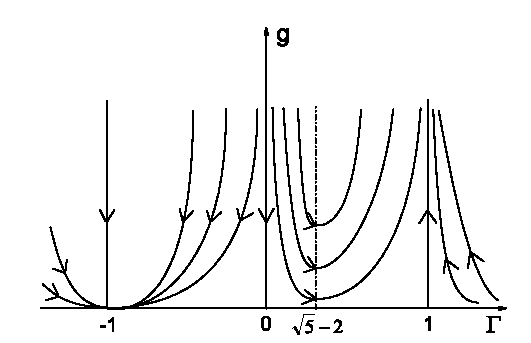
\includegraphics[scale=0.8]{rgflows.pdf}
	\caption{RG flow lines for the parameters $\Gamma$ and $g$ defined in the main body. 
	For the strongly anisotropic case $\Gamma < 0$ all flows go to the fixed point $\Gamma =0$ and $g=-1$. 
	For the weak isotropic case $\Gamma >0$, flow lines tend to $\Gamma =1$ and $g = \infty$ \cite{PhysRevLett.111.088701}. }
	\label{fig:rgflows}

\end{figure}

In practice, only the weakly anisotropic regime is accessible in the case of incoherent pumping \cite{2015PhRvX...5a1017A}, whereas for the OPO pumping it is experimentally viable to traverse different regimes by the adjustment of the pump strength. We shall now describe the various possible regimes for both pumping types and for both anisotrpic and isotropic parameters. 

In the weakly isotropic case, a dual modified electrodynamic theory has been mapped from the KPZ equation which describes the vortices as charges, extending the mapping that was used in the BKT transition. In the present case, the interactions of these vortices have repulsive contributions that grow with $\lambda$. Thus it was determined that beyond a length scale $L_v = e^{2\pi/\lambda}$, vortices are screened and thus always proliferate. Beyond this distance they are expected to show exponential correlations, while beyond the KPZ distance $L_{\text{KPZ}}$ stretched exponential correlations are expected, i.e. $e^{-r^{2\chi}}$ is the form of the correlation function, with $\chi \sim 0.39$ determined from numerical investigations.

In the case of incoherent pumping in the isotropic regime it is found \cite{2015PhRvX...5a1017A} that although in the thermodynamic limit the algebraic order will always be destroyed, the size $L_{\text{KPZ}}$ to which a finite system can show algebraic correlation depends on a tuning parameter $x = \gamma_p/\gamma_l - 1$ where the $p$ and $l$ are pump power and loss, respectively. Algebraic correlations may be destroyed in one of two ways: for a sufficiently large tuning parameter and system, decreasing the tuning parameter increases the nonequilibrium fluctuations so that the system enters the KPZ phase. Alternatively, a BKT transition may take place first. This is illustrated in \fig{\ref{fig:incoherentkpz}}.
It is noted that the KPZ length scale $L^*$ is much larger than realistic system sizes, and therefore may not be observed for incoherently pumped systems. 

\begin{figure}[htbp!]
	\centering
	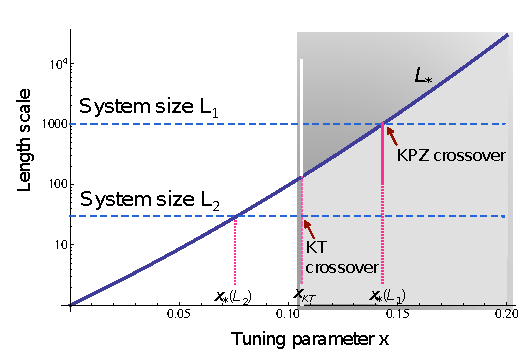
\includegraphics[scale=0.7]{incoherentkpz.pdf}
	\caption{The different regimes the system is in in the case of incoherent pumping depends on the tuning parameter $x$ and system size. At a combination with a sufficiently small system size and sufficiently large $x$, the system displays algebraic correlations. Depending on the system size, decreasing $x$ can lead to stretched exponential correlations either through entering the KPZ phase or via a BKT transition \cite{2015PhRvX...5a1017A}.}
	\label{fig:incoherentkpz}
\end{figure}

For coherent pumping, the length scales as a function of the pump strength relative to the maximum pump strength that allows the OPO regime is shown in \fig{\ref{fig:coherentwa}}. Although the length scale $L_v$ is less than that of $L_{\text{KPZ}}$ where the KPZ phase would be observable, thus seemingly precluding the KPZ phase, it has been pointed out that in numerical studies of up to 1000 $\mu$m that the vortex rich phase appears absent XX, which could suggest a prevention of the vortex proliferation, or an underestimation of $L_v$.

\begin{figure}[htbp!]
	\centering
	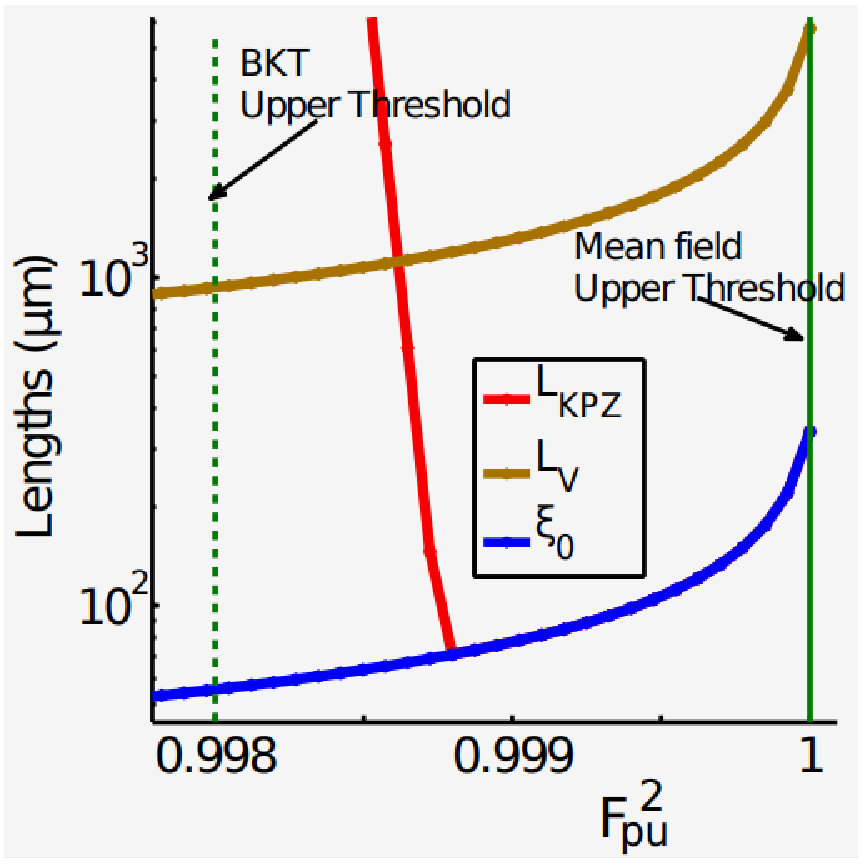
\includegraphics[scale=0.4]{coherentwa.pdf}
	\caption{The case of coherent pumping in the weak anisotropic regime. This shows the various length scales as a function of the pump power normalised to the maximum pump that allows the OPO regime. For most values of pump power the $L_v$ is less than that of $L_{\textrm{KPZ}}$ where the KPZ phase would be observable \cite{PhysRevX.5.041028}.}
	\label{fig:coherentwa}
\end{figure}
In systems with strong anisotropy there only exists a phase transition between the BKT phases \cite{2015PhRvX...5a1017A, PhysRevX.5.041028}. An incoherent pump phase diagram that illustrates this is shown in \fig{\cite{fig:incoherentanisotropic}}. In particular, the system exhibits ‘reentrance’ which means that by increasing the pump power it is possible to enter into the algebraic regime, and then subsequently exit it on further increase. Coherent pumping displays similar phases as the incoherent pump, specifically in reentrance, however in experimental realisations the various regimes can be explored much more easily with the available system size by varying the detuning (the energy difference between the cavity resonance and exciton energy at $k=0$), pump power, and pump wavevector. 

\begin{figure}[htbp!]
	\centering
	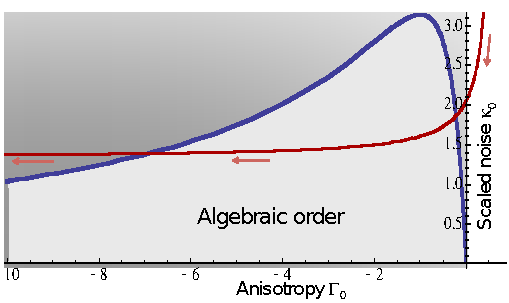
\includegraphics[scale=0.7]{incoherentanisotropic.pdf}
	\caption{A phase diagram for the anistropic KPZ state for the incoherent pump for the parameters $\Gamma_0$ (as defined in the text) and the parameter $\kappa_0 = \Lambda/\sqrt{D_x D_y}$ where $\Lambda$ is the noise strength. 
	The curve shows a potential route that would be traversed in experiment as pump power is increased: the key feature of reentrance where the algebraic phase is entered and left as this path is crossed \cite{2015PhRvX...5a1017A}.}
	\label{fig:incoherentanisotropic}
\end{figure}

\section{Project Aim}

The aim of the project will be to simulate the discretised KPZ equation on a finite lattice of phase angles in for various values of $\lambda$ both in the anisotropic regime and isotropic regime. The Binder cumulant will be plotted as a function of $(t/\log t)^{1/2}$, first to obtain the same collapse as in the study of the $XY$ model, then to test for the expected collapse in the anisotropic regime. The behaviour of the Binder cumulant will also be checked for in the isotropic regime. 

